\newpage
\section{Pianificazione}

Per migliorare lo sviluppo del progetto e rispettare le scadenze elencate al punto \hyperref[Scadenze]{1.6} di questo documento, lo sviluppo è stato suddiviso in sei periodi, ripartiti a loro volta in due macro periodi indicanti il primo, un periodo di investimento a carico del gruppo \Gruppo ed il secondo, facente parte del preventivo a carico dell'azienda proponente.

Periodo di investimento:
\begin{itemize}
\item \textbf{Analisi dei Requisiti};
\item \textbf{Analisi dei Requisiti in dettaglio}.
\end{itemize}
Periodo rendicontabile:
\begin{itemize}
\item \textbf{Prototipazione};
\item \textbf{Prototipazione in dettaglio};
\item \textbf{Progettazione finale e Codifica};
\item \textbf{Codifica in dettaglio, Validazione e Collaudo}.
\end{itemize}
Di seguito sono analizzati in dettaglio i periodi sopracitati e per ognuno di essi viene riportato il diagramma di Gantt; il diagramma riporta le milestone e le date di inizio e fine di ciascuna attività.

\subsection{Analisi dei Requisiti}
\textbf{Periodo}: dal 2018-03-03 al 2018-04-13 (RR)\\

Questo periodo comincia con la creazione del gruppo e si conclude con la consegna dei documenti per accedere alla Revisione dei Requisiti.\\
I documenti stilati e successivamente verificati durante questo periodo sono:
\begin{itemize}
\item \textbf{Norme di Progetto}: questo è il primo documento redatto in ordine cronologico poiché norma lo svolgimento di tutte le attività del gruppo \Gruppo; esso è indipendente dal capitolato scelto;
\item \textbf{Studio di fattibilità}: in questo documento vengono analizzati tutti i capitolati proposti. Per ognuno viene analizzato il dominio applicativo e tecnologico, valutandone i fattori positivi e negativi. È un’attività critica perché definisce il progetto sul quale il gruppo andrà a lavorare e blocca la stesura del documento di Analisi dei Requisiti;
\item \textbf{Piano di Progetto}: vengono pianificate tutte le attività necessarie allo svolgimento del progetto ed assegnate alle risorse disponibili, distribuendo il carico di lavoro in maniera uniforme;
\item \textbf{Piano di Qualifica}: vengono definiti gli standard qualitativi e le metriche da utilizzare per verifica e validazione;
\item \textbf{Analisi dei Requisiti}: viene effettuata l’analisi approfondita del capitolato scelto con lo Studio di Fattibilità e vengono identificati i requisiti obbligatori e facoltativi;
\item \textbf{Glossario}: contiene la definizione di alcuni termini utilizzati nei vari documenti, al fine di eliminare ogni possibile ambiguità di significato;
\item \textbf{Lettera di Presentazione}: documento che dichiara l’interesse del gruppo a partecipare alla gara d’appalto.
\end{itemize}

\begin{figure}
	\centerline{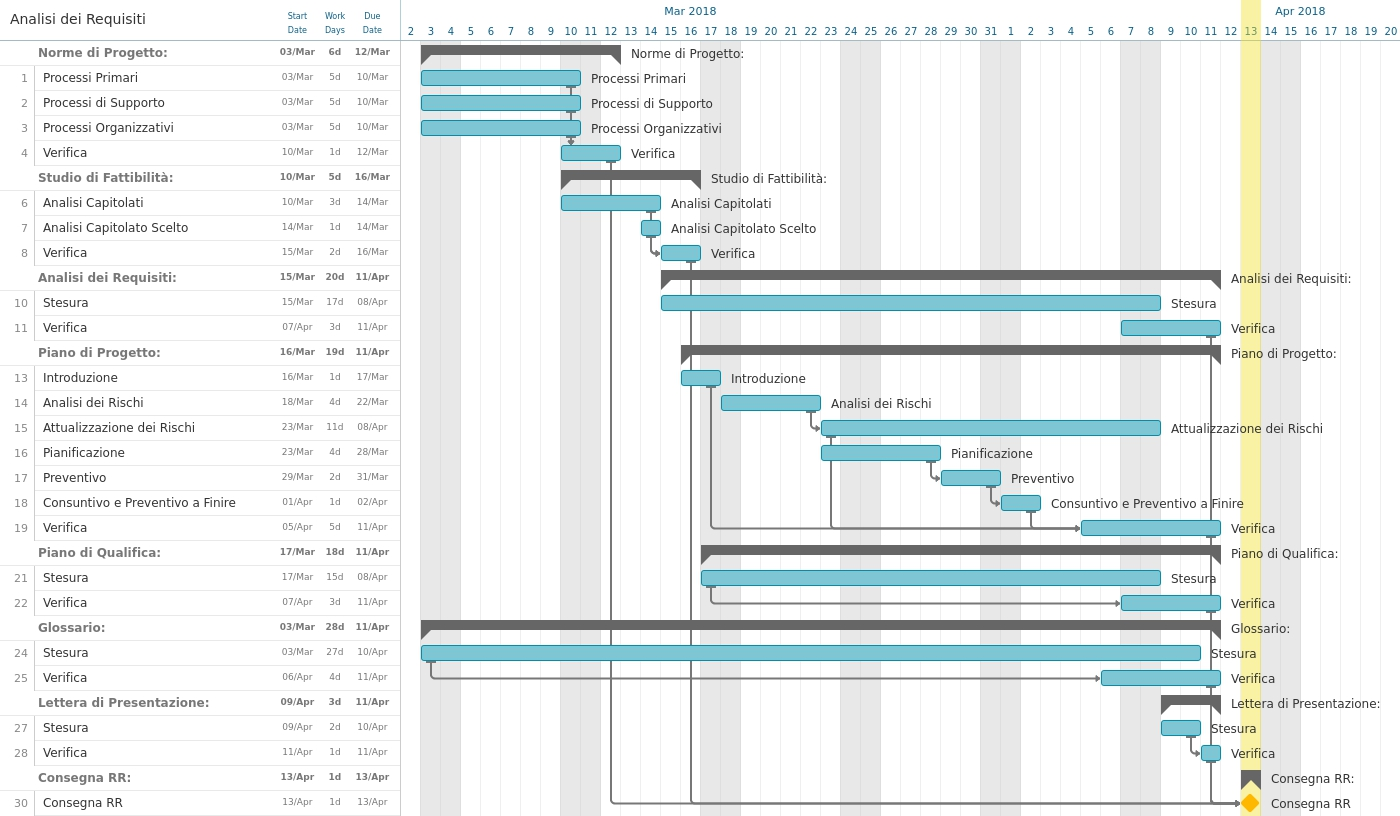
\includegraphics[scale=0.4]{img/DiagrammiGantt/AnalisiRequisiti.jpg}}
	\caption{Diagramma di Gantt: Analisi dei Requisiti}
\end{figure}
\clearpage

\subsection{Analisi dei Requisiti in dettaglio}
\textbf{Periodo}: dal 2018-04-14 (RR) al 2018-04-26 (Milestone Interna)\\

In attesa dell'esito della Revisione dei Requisiti, i membri del gruppo si impegnano a colmare le proprie lacune tecnologiche necessarie allo svolgimento del progetto. Parallelamente, si mira a consolidare ed ampliare i requisiti richiesti dal sistema e a migliorare il documento di Analisi dei Requisiti attuando le correzioni in base all’esito della Revisione dei Requisiti; vengono inoltre corretti e verificati anche gli altri documenti. Il termine fissato per la conclusione di questa fase corrisponde ad una milestone interna.\\ 

\begin{figure}
	\centerline{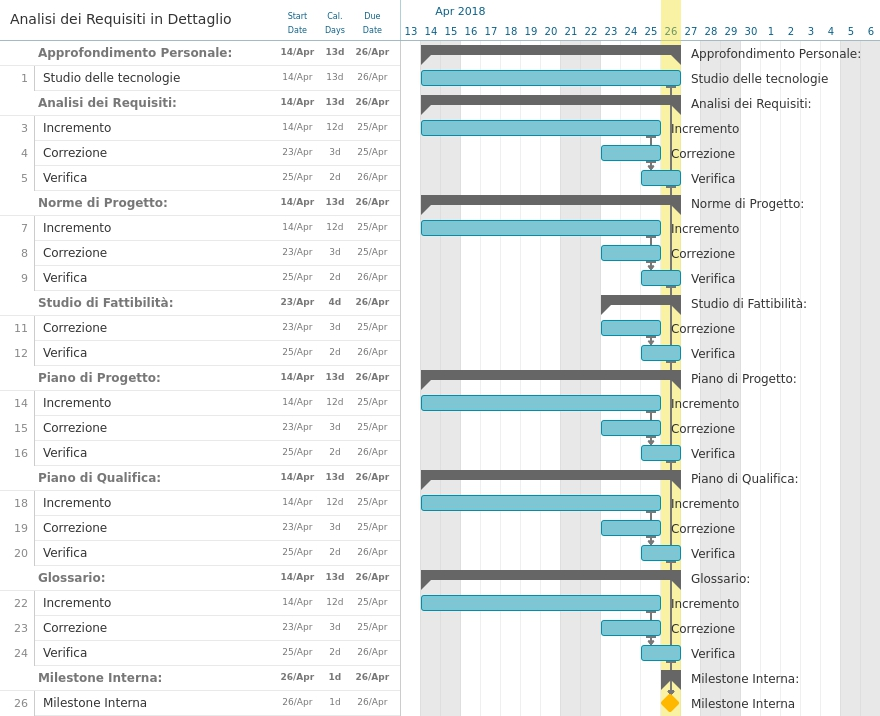
\includegraphics[scale=0.5]{img/DiagrammiGantt/AnalisiRequisitiDettaglio.jpg}}
	\caption{Diagramma di Gantt: Analisi dei Requisiti in Dettaglio}
\end{figure}
\clearpage

\subsection{Prototipazione}
\textbf{Periodo}: dal 2018-04-27 (Milestone Interna) al 2018-05-07 (RP)\\

Questo periodo è caratterizzato dalla realizzazione di un prototipo utilizzando le tecnologie necessarie, sulla base delle scelte del gruppo \Gruppo e delle richieste del proponente.
Lo scopo è quello di comprendere pienamente il dominio tecnologico del progetto e realizzare i casi d'uso ritenuti più importanti e significativi per la buona riuscita del prodotto finale, realizzando così una Technology Baseline. \\ 
Come attività di supporto si incrementano i documenti già redatti nei periodi precedenti.\\
Per semplicità si considera come periodo di consegna e presentazione della Technology Baseline la data di Revisione di Progettazione; sarà poi specificata una scadenza più precisa in fase di sviluppo. \\

\begin{figure}
	\centerline{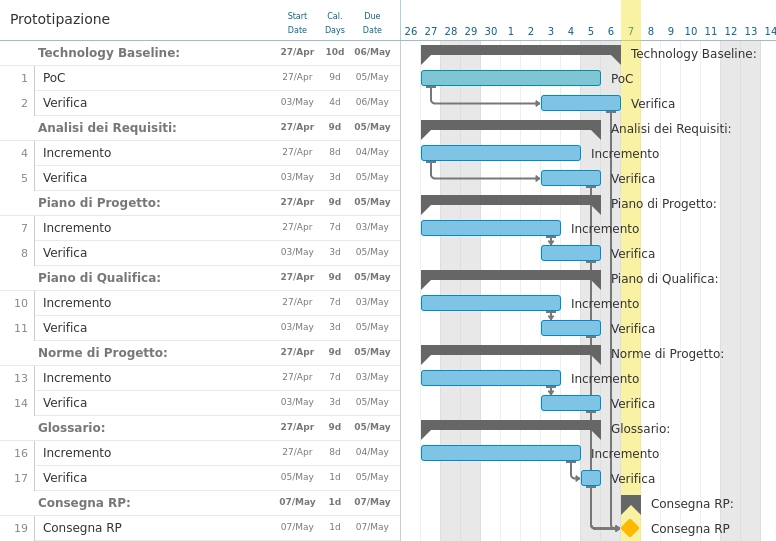
\includegraphics[scale=0.5]{img/DiagrammiGantt/Prototipazione.jpg}}
	\caption{Diagramma di Gantt: Prototipazione}
\end{figure}
\clearpage

\subsection{Prototipazione in Dettaglio}
\textbf{Periodo}: dal 2018-05-08 (RP) al 2018-05-16 (Milestone Interna)\\

In attesa dell'esito della Revisione di Progettazione, si incrementa la PoC finora realizzata, migliorando i requisiti già interessati. In seguito verranno effettuale le dovute correzioni a questa e ai documenti in base all'esito della Revisione di Progetto. La conclusione di questo periodo corrisponde ad una milestone interna.\\

\begin{figure}
	\centerline{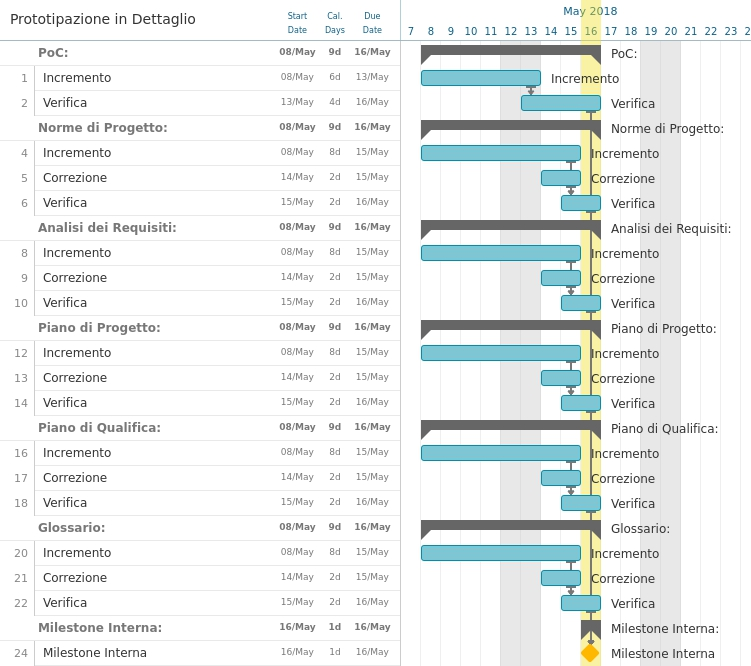
\includegraphics[scale=0.5]{img/DiagrammiGantt/PrototipazioneDettaglio.jpg}}
	\caption{Diagramma di Gantt: Prototipazione in Dettaglio}
\end{figure}
\clearpage

\subsection{Progettazione finale e Codifica}
\textbf{Periodo}: dal 2018-05-17 (Milestone Interna) al 2018-06-08 (RQ)\\

Si procede con la progettazione in dettaglio dell'architettura sistema, comprensiva di design pattern implementati e diagrammi delle classi e di sequenza; il risultato di questo insieme di attività comporrà la Product Baseline del prodotto. Una volta definita, si procede con la fase iniziale di codifica per realizzare i requisiti obbligatori stabiliti in precedenza, riutilizzando ed ampliando il codice prodotto durante la fase di Prototipazione e Prototipazione in Dettaglio. \\
Come attività di supporto si incrementano alcuni documenti già redatti nei periodi precedenti e si stilano due nuovi documenti:
\begin{itemize}
	\item \textbf{Manuale Utente}: contiene indicazioni utili all'utente finale per l'utilizzo del prodotto
	\item \textbf{Manuale Sviluppatore}: contiene indicazioni utili allo sviluppatore per la manutenzione e l'incremento del prodotto
\end{itemize}
Per semplicità si considera come periodo di consegna e presentazione della Product Baseline la data di Revisione di Qualifica; sarà poi specificata una scadenza più precisa in fase di sviluppo. \\

\begin{figure}
	\centerline{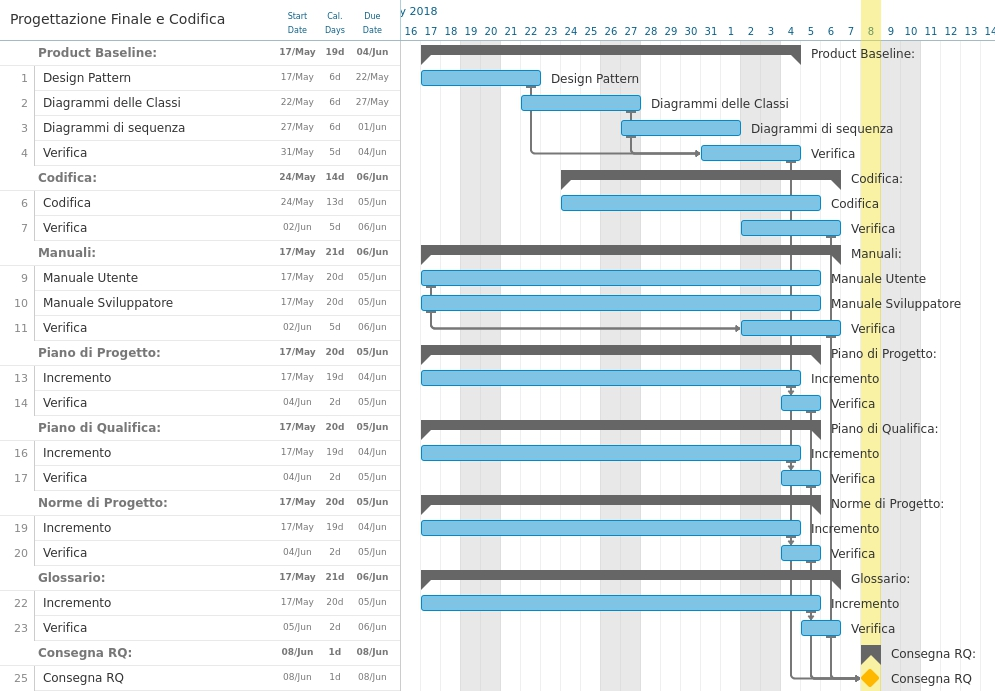
\includegraphics[scale=0.5]{img/DiagrammiGantt/ProgettazioneFinaleCodifica.jpg}}
	\caption{Diagramma di Gantt: Progettazione Finale e Codifica}
\end{figure}
\clearpage

\subsection{Codifica in Dettaglio, Validazione e Collaudo}
\textbf{Periodo}: dal 2018-06-15 (RQ) al 2018-07-15 (RA)\\

Durante quest'ultimo periodo di sviluppo, si incrementano i documenti redatti finora e si effettuano gli ultimi incrementi di codifica; a seguito di queste attività si procede con la verifica del sistema completo e il collaudo di esso.

\begin{figure}
	\centerline{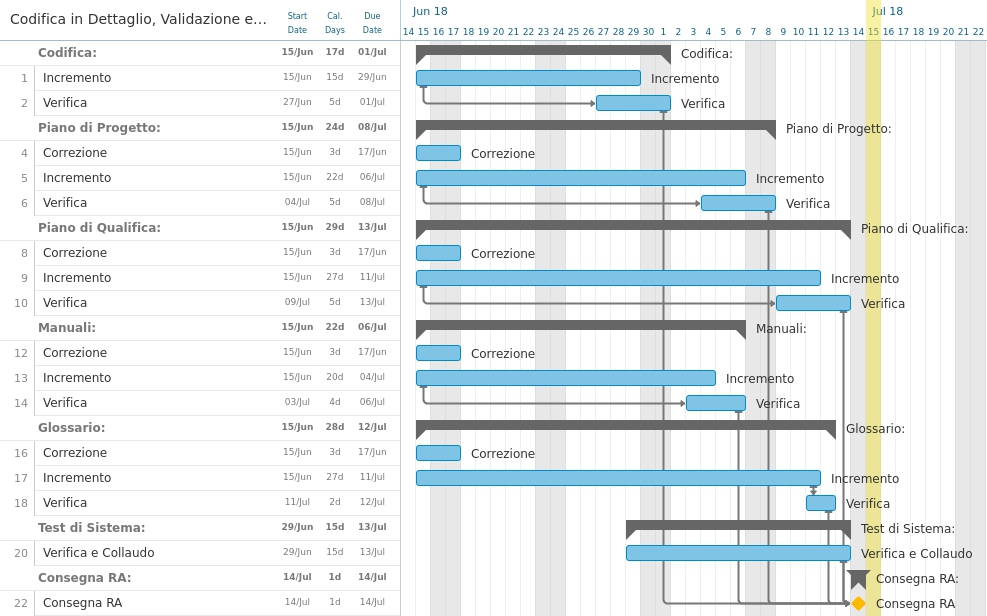
\includegraphics[scale=0.5]{img/DiagrammiGantt/CodificaValidazioneCollaudo.jpg}}
	\caption{Diagramma di Gantt: Codifica in Dettaglio, Validazione e Collaudo}
\end{figure}
\clearpage
